\documentclass[a4paper]{ctexart}

\usepackage{
    amsmath,
    amssymb,
    graphicx,
    minted,
    fontspec
}

% \setmonofont{Fira Code}
\setminted{breaklines, showtabs=false}

\pagestyle{plain}

\title{基于启发函数对穿越沙漠游戏的决策模型}
\author{}


\begin{document}

\maketitle
\zihao{5}

\begin{abstract}
本文通过建立数学模型,根据不同情况下的条件设定变化,对穿越沙漠小游戏进行多方面多角度的考量分析,以确定出最优的游戏策略,使得最大化满足游戏目标,即在规定时间内到达终点,并保留尽可能多的资金。

本文在模型建立上使用了一种完全原创的动态决策方式,借鉴了 A* 寻径算法利用启发函数的技巧。启发函数将获取信息的手段从深度搜索,替换成了在局部的大体估计,大量缩减了估计出优解所需要的计算量和信息量。

A* 算法的行为主动的缩减了决定行进方向所需要的信息量。而在无法获取全局统筹信息,只能观察临近限制条件的情况下,也同样可以利用启发函数的思想。

将在决策之中影响决策的关键参数抽象出来之后作为启发函数的输入。在周边的可选决策之中,选择能够使得决策实行之后状态的启发函数值,是各个可选决策中最大(根据需要,也可能是最小)的一个。

根据问题的不同,抽象出来的参数可能不同,修改适当的启发函数可以让算法立即适应新的环境。

这样的启发式决策过程的主要决策倾向就体现在决策函数一个内容中,这赋予了启发函数思想极大的自由度。

本文将会给出一个对具体问题构造的启发函数,生动的描述作者们如何考虑决策过程之中各个参数的变化。

在前四关的处理中,本文通过进行手动的推演,不断微调某些事件持续的时间,调整某些事件的前后顺序,观察对于最终盈余的影响,总结出了多条能够指向更高收益额的准则;对于第三大题所要求给出的一般策略,由于每一种天气组合都会推出一种可行的最优解,只能通过贪心算法进行寻路或是深度学习来完成,且程序复杂度极高,运行速度慢;对于第三关多人进行宏观规划与实时博弈,从n=2,3等低人数最优规划进行分析,采用数学归纳法的思维,逐步将n为较大值时分解为更低人数的方式进行讨论,模拟一二题给出类似的准则,大大缩减了程序模拟时的复杂度。

\textbf{关键词:}动态规划、启发函数、决策优化、博弈论
    \end{abstract}

\clearpage

\section{问题背景}

当前时代背景下,AI在各类需要高智能参与的场景中体现了重要的作用,面对实时出现的不同场景,需要在尽可能短的时间内给出应对,广为人知的Alpha Go在围棋这一实时策略游戏中展现出了极高的智能。生活中许多复杂的选择问题,人工智能能够为我们做出更理性的选择,本道题以沙漠生存为大背景进行沙盘推演,给出了各种限定条件与最终目标,需要考虑到博弈与宏观规划给出最优路径,在较少的影响因素下模拟人工智能的决策过程。

\section{问题重述}

本题主要围绕给定限制条件下,动态变化的环境中如何进行更优决策展开问题。

动态演变的环境条件主要是天气,玩家即使进行相同的活动,在不同天气下需要负担的成本却是完全不同。

第一问给出了变化的限制条件的全局规律,如何在这样的信息背景下,用好全局条件,进行更好的统筹,让玩家能够争取利益最大化?

第二问将随时间动态变化的条件规律掩盖,玩家如何在仅仅知道自身当前保有的资源,和所处位置的情况下,既成功通过沙漠,又尽可能地利用动态决策增加金钱的积累量?

第三问,加入了不同个体之间的交互过程,场地的限制因素被进一步扩大。第一、二问中,地图仅仅涉及到玩家如何在不同区域之间进行性移动和决定行为,第三加入了如何在地图中分布各个玩家,充分利用在第一、二问之中被忽略的区域,某种程度上是使得玩家们利益最大化?

本次的讨论将会围绕这三个问题进行讨论。

\section{问题分析}

\subsection{问题一的分析}

问题一要求在只有一名玩家且在整个游戏时段内每天天气状况事先全部已知的条件下,通过对游戏基本规则的解读及其他方面的分析,简化地图,给出玩家的最优策略,并求解出附件中的“第一关”和“第二关”的结果,最终补全相关文件。故本文首先用将较为简单的地图进行模型化分析,简化地图行进方案,从而得出相关结果,补全表格数据。

\subsection{问题二的分析}

问题二要求在问题一的基础上,在只有一名玩家且仅知道当天的天气状况的条件下,通过问题一所给出的解决方案,进行进一步的条件适用性优化,来决定当天的最佳行动方案,并对附件中的“第三关”和“第四关”进行具体分析。故本文在考虑多方面因素后,给出以下评价指标:  通过较为全面的评价,最终得出相关模型的分析结果,为后续工作打好基础。

\subsection{问题三的分析}

问题三要求在问题一和问题二的解决基础上,增加人数条件及对应的资源消耗和资金消耗方法,通过建立启发函数和相关数学模型,对“第五关”和“第六关”分别进行具体分析,并给出合理的游戏策略。故本文就食物量、水量、截止日期、资金、天气情况等参数进行了数据的因子分析,构造出启发函数,并将如上影响因子加入函数中,通过函数的分析进行评估,从结果出发,给出最优的游戏策略。

\section{名词解释与符号说明}

文中图片使用 st 表示起点、ed 表示终点、v 表示村庄(village)、m 表示矿山(mine)。当地图之中出现多个相同类型的特殊结点,则使用下标进行区分。

食物和水数量的单位,若未进行特殊说明,均为箱。

\section{问题一的模型建立与求解}

\subsection{模型准备}
\subsubsection{对游戏基本规则的一般性解读}

游戏的核心目标是保证在规定时间内到达终点的前提下,去获取更多的资金。游戏总计有八条基本规则,具体分析可知该类题的主要限制因素是截止时间与满载的负重上限,而天气则是对路径规划的决策产生影响的核心因素。

本文对于第一、二关卡,首先在不同情况下通过手动模拟的方式进行分类讨论及分析,而后给出如下准则:

\begin{enumerate}
    \item 直接前往终点的路径为负收益,不符合上述获取更多资金的目标;在矿山的单日挖掘收益为1000元,挖矿收益高于任何天气条件下的挖矿资金消耗(沙暴日挖矿需花费资金450元,用以补充食物和水的消耗)。
    \item 在前往地图上任何特殊目标点(村庄、矿山、终点)的时候,走最短路径一定会有更高的收益;任何绕路的行为都会出现两倍的行进消耗,不符合利益最大化的目标。
    \item 天气条件已知的情况下,在确保存活的同时,尽量多在到达终点前挖矿可能可以带来更多收益。
    \item 在路过村庄时,由于在村庄无需停留即可购买水与食物,不会浪费时间,因而在经过时可以尽可能补充之后所需的水与食物两种资源,而没有其余代价。
    \item 在限制条件为30天的情况下,必然会出现中途食物耗尽的情况,即在出发时要尽可能满载,以保证到达补充点时资源的充分利用,能用剩余的负重盈余尽可能的购买食物。相比较而言,食物单箱的重量相对轻且基准价格高,这意味着如果食物耗尽后,后续在村庄补充时,每箱食物将多付出10元,而后续补充每箱水的价格只需多付出5元,故可在起点多购买一些食物,以节省资金。
    \item 在明确天气状况的条件下,沙暴天气来临的同时玩家在矿山,此时有原地等待与挖矿这两种选择,其在矿山挖矿获得收益的期望E更高,故通常选择挖矿。
\end{enumerate}


\subsection{模型建立}

在本题的地图之中,区域的大小、形状并不影响讨论的结果。影响讨论结果的只是各个区域之间的邻接情况。所以本题的地图可以完全使用一个无向图来进行描述。

同时在不同区域节点之间移动一次消耗的时间也完全相同,无向图的之中的边并不需要特别添加权重。

如果再进一步考量本题的游戏目标,即在规定时间内到达终点,并且尽可能多地保有金钱。也就是说,需要尽可能避免因为绕路而产生的资源消耗。抽象出来的无向图可以进一步简化。在地图中只有带有特殊功能的结点(起点、终点、村庄、矿山)必须要考虑,而其他的结点很大一部分是可以从地图中忽略的。

有一部分结点删除之后,并不会影响在功能性结点之间移动的最短路径长度。比如关卡 1 的地图之中,图 \ref{fig:stage1-shade} 中未标红的区域都可以忽略。

\begin{figure}[htpb]
    \centering
    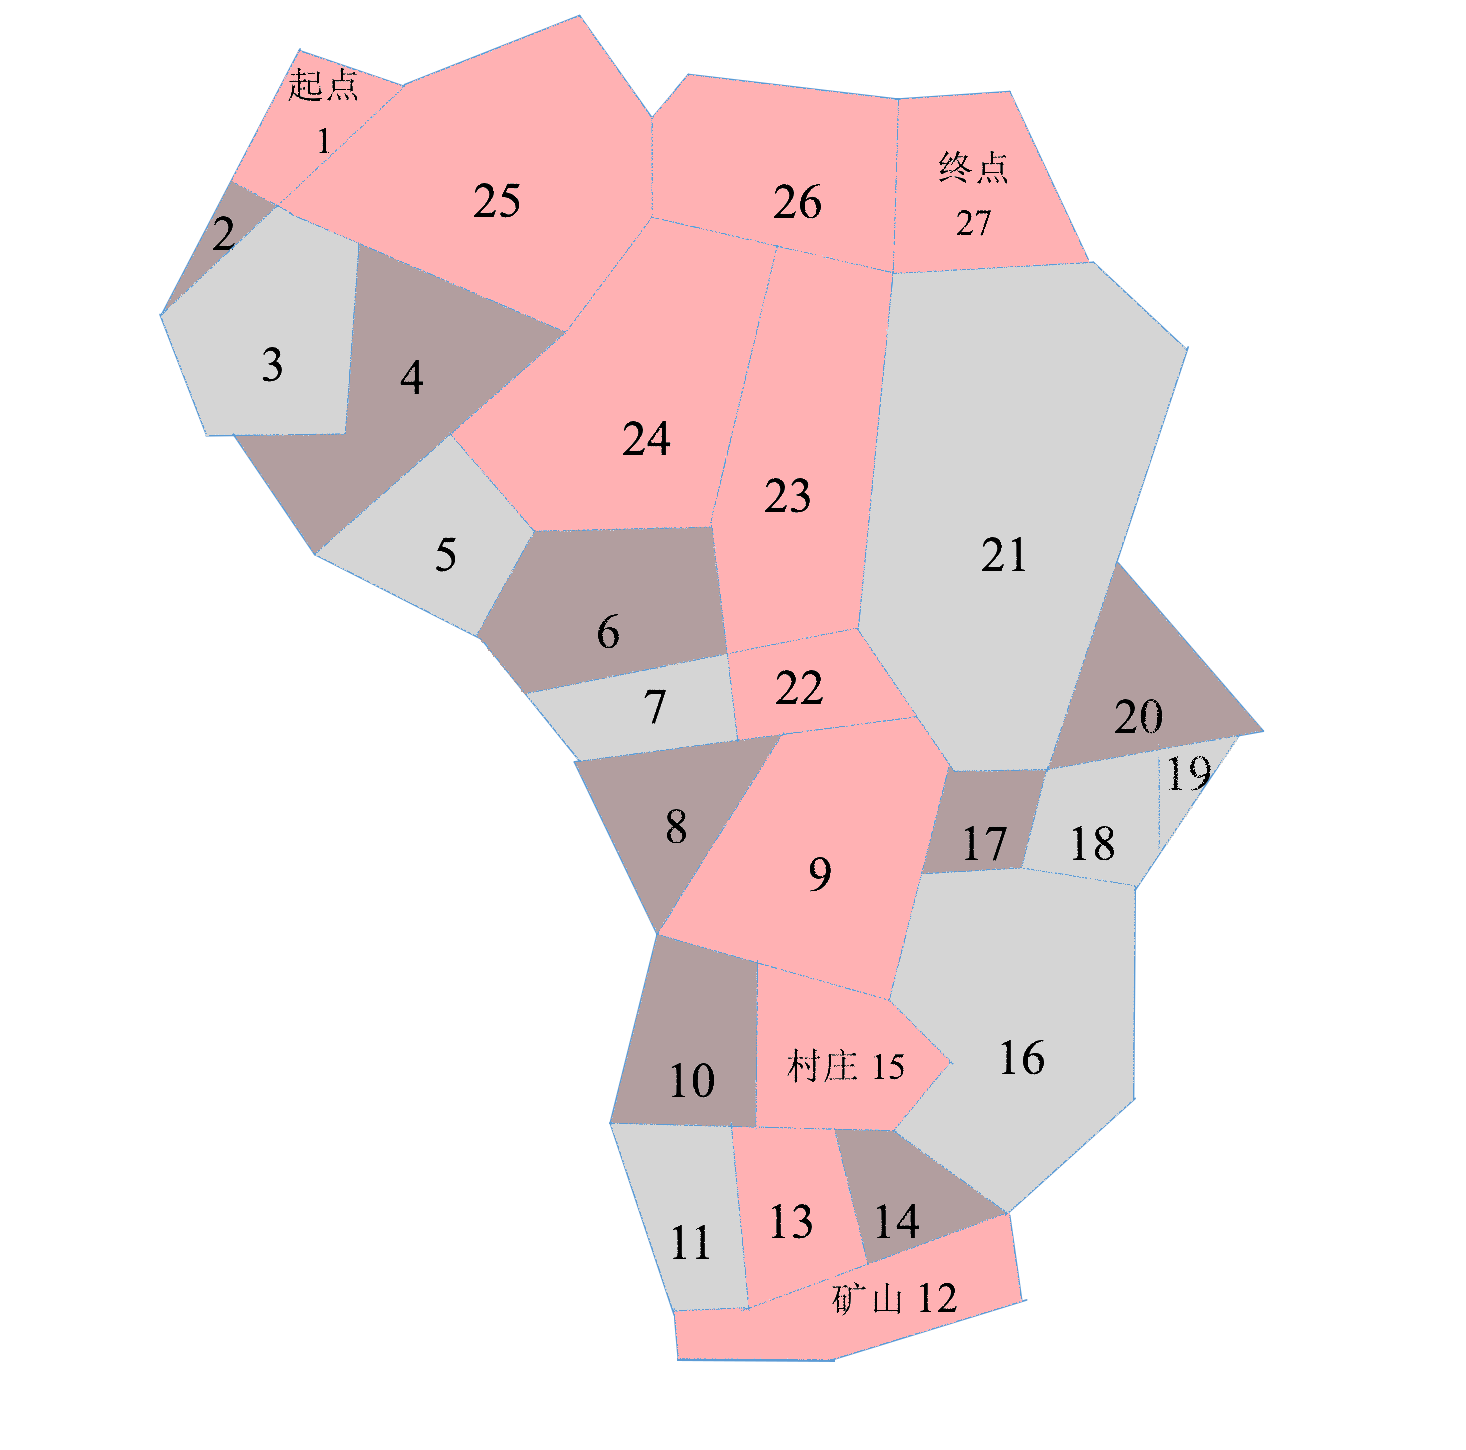
\includegraphics[width=0.5\textwidth]{./pictures/statge1_simple.png}
    \caption{未标红的区域均可以忽略}
    \label{fig:stage1-shade}
\end{figure}

地图可以大幅度简化——只考虑功能性结点,和功能性结点间一条最短路径上的结点,而为了在结点之间进行移动所需要的天数,会给无向图的边进行附权。图 \ref{fig:simplified-1-and-2} 是关卡 1 和关卡 2 的地图在经过简化之后得到的。

图 \ref{fig:simplified-1-and-2} 中红的字样为边权。

\begin{figure}[htpb]
    \centering
    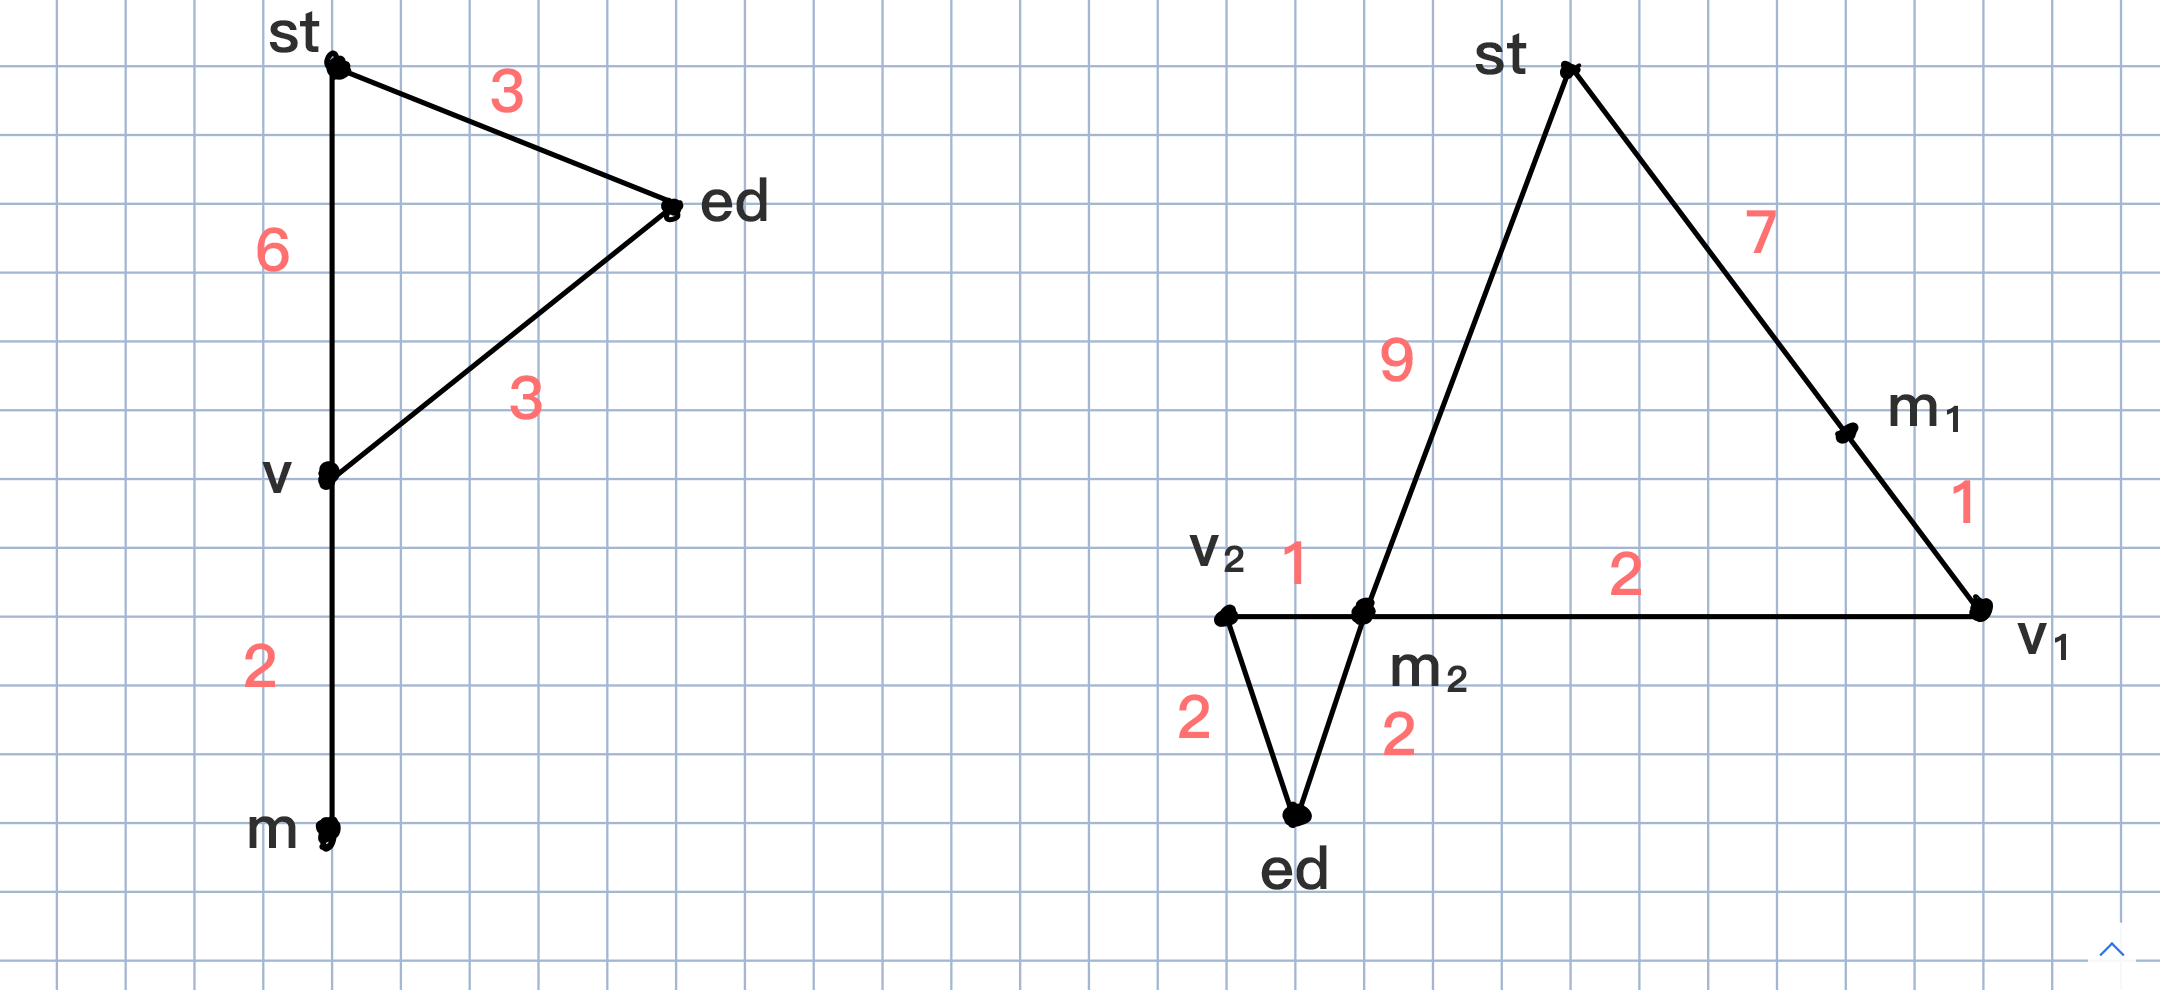
\includegraphics[width=0.8\textwidth]{./pictures/simplified.png}
    \caption{关卡一、二地图抽象的最终结果}
    \label{fig:simplified-1-and-2}
\end{figure}

本队程式化了整个行进过程,通过命令行交互程序进行过程的模拟。\footnote{此程序同样也用在了第二问的启发式决策模型的验证当中。}

\begin{figure}[htpb]
    \centering
    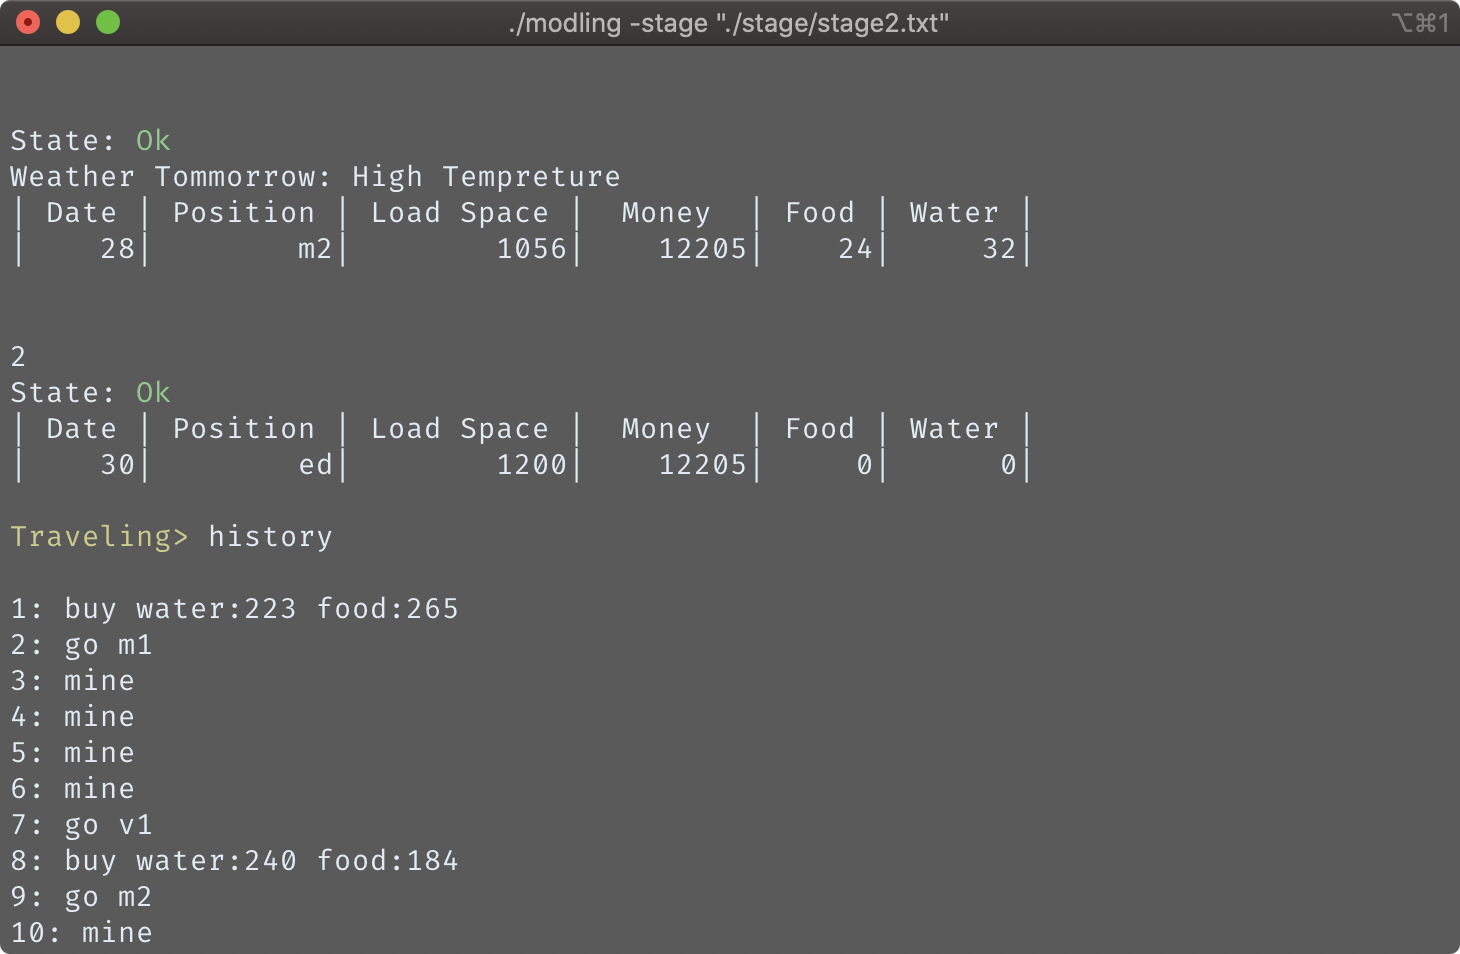
\includegraphics[width=0.8\textwidth]{./pictures/screenshot.png}
    \caption{程序运行截图}
    \label{fig:sscreenshot}
\end{figure}

\subsection{关卡一的分析与解}

本题将会使用图 \ref{fig:simplified-1-and-2} 之中使用的字母标记。

本关卡除去起点外,有三个功能性结点。优先不考虑直接去往终点,而在剩下的结点之中,从 st 去往 m 的最短耗时路径为 8。而在长度为 8 的 st 去往 m 的路径之中,包含有经过 v 的路径。

所以本关卡的第一步决策的目的地就被限制到了 v 一点。

在到达 v 之后,目的地变成 ed、m 两者。若选择直接去往 ed,则由于未进行任何赚取金钱的活动,收益不如直接从 st 去往 ed,进而淘汰该选项。可选决策也只剩下从 v 继续去往 m。

决策的分歧主要出现在到达 m 之后——在 m 进行挖矿之后,必然要回到 v 进行物资的补给,补给结束之后是要回到 m 继续进行挖矿,还是直接去往 ed。

在 m 和 v 之间往返需要 4 天,在这样的一个时间跨度内,如果从 m 离开的时间不当,则可能在行进途中遭遇沙暴被困。与沙暴天进行挖矿作业相比,沙暴天被困在经济效益是非常不划算的;但是沙暴天选择不挖矿可以在资源不足时用于节省资源进行后续行进。

基于如此的认识,应当尽量避免 17、18 日的沙暴被困在行进途中。那么从 m 离开的时机主要在两个时间段:12 ~ 16 日之间、19 ~ 24 日之间。

由于 12 ~ 16 日之间如果离开 m 去往 v 进行补给,若是此后直接去往 ed 则由于挖矿时长不够而影响最终的经济收益;若是再次回到 m 进行挖矿,则会由于离开过早,资源消耗量不够,载重空出的部分较少而使得补给量受限,影响回到 m 之后挖矿的续航能力。故此段时间离开应当是经济效益最低的,后续通过程序验证也的确如此。

如果 19 ~ 24 日间离开,则离开的日期受到前置的资源分配的影响。如果到达 v 之后可以直接去往 ed,也可以再次去往 m。如果再次去往 m 则为了尽可能利用好 25 日出现的沙暴天气,动身离开 m 去往终点的日子应当是 26 日。

接下来考虑如何进行资源分配的问题。资源分配可以通过确定的行程安排,从终点进行逆推计算。以经过村庄作为行程的分段,逆向从终点根据行为推算在每个补给点应当保有的最小资源数量(最小是为了保证在行程结束后没有资源剩余)。

最终通过演算得到的一个金钱剩余为 10430 的行程安排。

\begin{enumerate}
    \item 在 st 购入 180 箱水,330 箱食物。
    \item 去往 v。
    \item 购入 163 箱水。
    \item 去往 m。
    \item 连续挖矿 7 天。
    \item 18 日什么也不做,节省生存资源准备后续行进。(这一天休息也可以放在 11 日或者 17 日的沙暴天)。
    \item 去往 v。
    \item 购入水 36 箱,食物 19 箱。
    \item 去往终点。在 23 日的行程结束之后抵达终点。
\end{enumerate}

\begin{figure}[htpb]
    \centering
    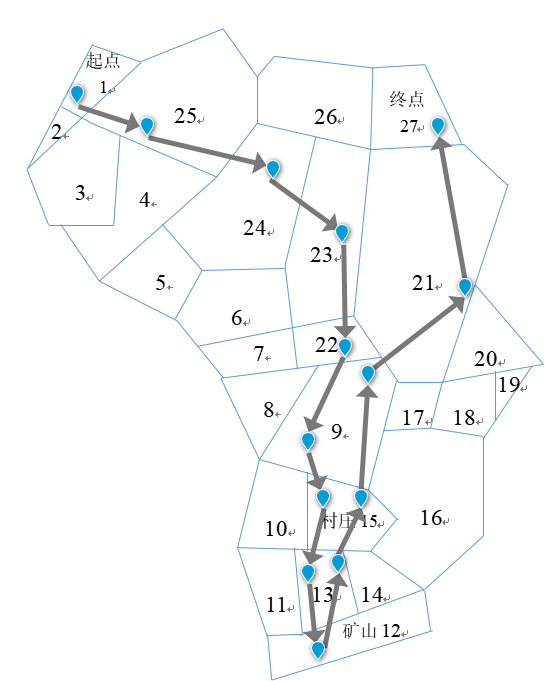
\includegraphics[width=0.6\textwidth]{./pictures/route.jpg}
    \caption{路线图}
    \label{fig:./pictures/route.jpg}
\end{figure}

\subsection{关卡二的分析与解}

首先,利用上述简化图像的方式,得到图 \ref{fig:simplified-1-and-2} 中右侧的关卡二缩略图

本题将会使用图 \ref{fig:simplified-1-and-2} 之中使用的字母标记。

本关卡除了起点以外总共有五个特殊结点,有两组村庄与矿山处于距离为1的相邻位置,两组特殊结点都距离终点较近,距离起点较远,经计算第一次到达特殊结点后无法维系长时间的挖矿,必然会在17号前需要进行一次补给

相比而言,m1比m2距离终点更远,且从m1返回v1是在远离终点,所以可以认定v1与m1之间不应该进行往返行为,选择v1走向m2会带来更高的潜在收益

st前往v1的路径上必然经过m1,有以下两种选择:

\begin{enumerate}
    \item 停留m1利用沙暴日挖矿,前往v1补给后再前往m2
    \item 在m1不做停留直接前往v1,补给后前往m2
\end{enumerate}

\begin{figure}[htpb]
    \centering
    
\includegraphics[width=0.8\textwidth]{./pictures/flowchart.jpg}
    \caption{对关卡二的决策进行流程分类讨论}
    \label{fig:flowchart}
\end{figure}

对于方案一,第九天末到达m1,总载重允许其挖掘到13号,前往v1,这个过程总共消耗了223箱水与209箱食物,按照准则5,初始的资源携带方式应该为:223箱水,265箱食物;m1出发利用14-16三个高温天进行行进到m2,期间经过v1进行补给,这种行进选择符合准则7,同时避免17-18由于沙暴天气困在路上而浪费时间,到达m2后接下来有两种方案。


\begin{enumerate}
    \item 选择不往返而是耗尽存量之后直接前往终点(前往终点中途可经过村庄)。
    \item 往返在v2与m2之间,尽可能的提高挖矿天数,最后一次准备足量资源前往村庄。
\end{enumerate}

方案1.1的配重余量只允许从事挖矿到23号,直接前往终点最后的金额为12165;

方案1.2按照准则在可取条件下选择高温天进行v2与m2之间的行进,经计算19-20往返后续连续挖矿所需要的总配重加上最后直接前往终点的资源重量之和不超过负重上限。这种形式的方式下第一次v1下的补给为184箱食物,与240箱水,第二次19号到达v2进行补给量为69箱水与63箱食物,挖矿至28号,前往终点,最终剩余量为0水0食物,按照这种方式且将所有的行进都放在高温天,没有浪费任何一天时间进行停留,达到方案1.2到达m2后进行一次补给往返的理论最大值,为12205;

接下来考虑方案2中的情况,不在m1进行任何的停留,直接前往v1,这种情况下虽然由于11号的沙暴天将不得不困在路途中,但由于从起点到v2所在处距离相对远,必然会很快的面临补给,路过补给要比往返补给来的省时,同时,通过st-v1-m2的路径总长为10,而通过路径st-v2-m2的路径总长为11;因此这种条件下因沙暴停留一天比之在晴天或是高温条件下行进一天消耗更少,选择前者更为有利。与方案1相同,也有直接前往终点与往返补给两种选择,但简单的计算可知,同方案1一样,直接前往终点一定会导致更低的收益。故我们方案2的可行后续方式为:选择合适日期进行往返v2进行补给,最后由矿山直接前往ed.

此时的最优解依旧基于准则7,选择购买405箱食物,130箱水,直接前往v1,此时剩余的食物为283箱,水全部耗尽,补充211箱的水达到满载,前往m2,于13号到达矿洞,14-18号进行挖矿获取资金,基于准则7,与19-20号两个高温天进行v2之间的往返,补充86箱食物,174箱水,此时剩余资金为4730元,20号晚回到m2,21-28进行八天挖矿获取资金,最后直接前往终点,终点耗尽所有水与食物,此时最终的资金为12730元.

最终通过演算得到的一个金钱剩余为 12730 的行程安排。

\begin{enumerate}
    \item 在 st 购入 130 箱水,405 箱食物。
    \item 去往 v1。
    \item 购入 211 箱水。
    \item 去往 m2。
    \item 连续挖矿 5 天。
    \item 19 日去往v2
    \item 购入 86 箱食物,以及 174 箱水。
    \item 去往m2。
    \item 连续挖矿 8 天。
    \item 去往终点。在 30 日的行程结束之后抵达终点。
\end{enumerate}

\section{问题二的模型建立与求解}

\subsection{模型准备}

\subsubsection{A* 算法}

A* 算法是在定态地图之中寻找从给定起点到给定终点尽可能短的路径的寻径算法,算法中每一次迭代会以当前位置为中心对邻接的位置进行评估,这个过程中会使用启发函数大致估计对被探索的点与终点间剩余的距离。选取邻接点中启发估计值与到达该结点需要的距离只和最小的一个,作为下一步的落脚点。

\subsubsection{启发函数从寻路迁移到决策}

使用启发函数的过程只是在当前点对各个可以到达的邻接结点进行估计,使用的信息只有当前所在结点的情况以及当前结点和终点之间的位置关系,不需要在某一个方向上连续进行更多的深度搜索来进行当前位置的角色。

同时,对于不同的具体情况,选取适当的启发函数可以很大程度上辅助探索的进行。比如若已知障碍物主要延坐标系中斜率为 1 的方向分布,则启发函数可以选取在斜率为 1 的方向上取较小值,而在斜率 -1 方向上取得较大值的函数来描述这样的地图中的寻径过程。因为在这样的地形中,顺着斜率为 1 的方向走较少遇到障碍物,需要绕路的可能性更小,理应是更划算的方向;而 -1 的方向上更可能被阻碍,应该是较少选择的方向,所以启发函数在这个方向上应该有更大的值。

在本题当中,玩家只能知道当天的天气,没有能力对天气信息进行估计。能够使用的信息只有当前自身的资源储量、当天的消耗、当前位置和其他功能性结点之间的距离,出于信息的限制,本文中欲将启发函数迁移到本题中,根据对于不同的模型假设(比如已知第四关中沙暴发生概率很低)对于启发函数

\subsection{构建游戏方案}

\subsubsection{一般性启发式模型的构建}

当每天只能知道当天的天气,进行决策的单位必须需要缩小到一天。不能再同关卡一、二一样以在功能性结点之间进行一次移动为主要决策单位s。例如在此题设中,可能会出现决定前往矿山并行进一天后若突然遭遇沙暴天气,随后立即终止行程直接前往终点的情况。

此模型在进行决策的过程之中,需要依赖预先假设的天气分布概率,天气的恶劣成都会在决策使用的启发函数中有一定的体现。

更进一步,如果希望以保守的方式——即高生还率——为目标通过此次沙漠穿越,则可以将天气概率模型中恶劣天气的概率调高。理想的决策启发函数在这种情况下,应该对物资的减少更为敏感,随着物资的减少快速地体现出“尽快走向终点”的决策倾向。

经过思考,对启发函数应该需要有如下的一些性质:

\begin{itemize}
    \item 能够一定程度上反映走向一个区域的潜在经济收益。
    \item 能够对当前的资源持有程度有反应,当资源量减少时,走向村庄/终点的决策倾向会逐渐体现。
    \item 经济收益参数会与生存率感知相互作用,在资源相对充足是会对有趋利倾向,而在生存被保障的程度降低时,经济则会较难吸引玩家。
    \item 对剩余的天数有感知,大多数时候旅行天数都是充足的,此时感知天数的指标变化平缓;当剩余天数不足时,该指标则会快速变化,短时间内超越经济考量使得通向终点成为主要目标。
\end{itemize}

本文决定使用概率模型来对生还保障程度进行估计——为了判断当前的资源是否足以保障生存,需要知晓从当前位置到达补给点/终点的资源消耗期望。

这样的期望值可以通过蒙特卡罗式的方法进行求解,按照在模型建立之初给定的各种天气发生的概率随机生成一组天气。使用这组天气计算地图中所有结点到达 m、v、ed 所消耗的资源数量,这样的操作重复多组,使用数消耗数量的平均数作为消耗的基准值(期望值)。在当前资源数量超过基准消耗值时,认为使用当前的资源足以保障到达目标结点。

$t$ 记当前行程剩余的天数,$t_{ed}$ 表示被选中的结点距离。

$a_f$、$a_w$ 表示从当前位置行进到选中邻接结点之后食物和水的剩余量,$E_f$、$E_w$ 分别表示被选中的邻接结点去往最近村庄需要的食物量和水量的期望值与去往终点需要的食物量和水量期望值中较小的一个。

$d_m$ 表示被选中结点去往最近矿山的最短路径长。

本文尝试给出一种构造启发函数的方式。考虑如下三个指标:
\begin{align*}
    \omega &= \dfrac{k_1}{t - t_{ed} + l_1}\ (l_1 > 0)\\
    \alpha &= \dfrac{k_2}{a_f - E_f + l_2} \cdot \dfrac{k_3}{a_w - E_w + l_3}\\
    \beta &= k_4 d_m + l_4
.\end{align*}

如果 $\omega$ 偏大,表示决策有较强的前往终点的倾向;如果 $\alpha$ 偏大,则表示有较强的由于资源不足而前往终点/补给点的倾向;如果 $\beta$ 较大,则说明当前的经济效应低。

三个参数均为越小越好。$\{k_i \mid i = 1, 2, 3, 4\}$ 与 $\{l_i \mid i = 1, 2, 3,, 4\}$ 均为常数。

在 $k_i$ 和 $l_i$ 确定之后,会使得分母数值变为负数的结点都是决策中一定不可以去的结点。

如果取较大的 $k_i$,则对应的指标对状态变化会更加敏感。

如果取较大的 $l_1$ 则表示决策对去往终点有更加急迫的倾向。

如果取较大的 $l_2$ 则表示对食物储量保障要求较为宽松,反之则代表对食物储量保障要求严苛。$l_3$ 类似。

如果取较大的 $l_4$ 则表示有较为强烈的赚钱欲望,反之则表示经济欲望弱。

取启发函数为 \[
    h(x) = \omega \cdot \alpha \cdot \beta, \text{x 为某一个结点}
.\]

在每一次决定第二天如何行动时,对当前结点的全体邻接点计算启发值,取启发值最小的一个作为下一步的落脚点。

\paragraph{如何决定购买资源时购买的数量} 当到达可以进行补给的位置(第零天的起点、旅途中经过的村庄)时,可以使用 $\beta$ 值的大小来决定购买多少资源。可以根据是情况,设计一个阈值,当 $\beta$ 过于此阈值时,选取使得 $\beta$ 值降低到阈值的花费最小的一种资源补给方式进行购买即可。\textbf{此阈值同样属于该模型的可调参数之一}。

\subsubsection{第三关题目分析}

首先分析第三关相较于第一二关题设条件的差异,与之相比,提高了高温天气对于水和食物的消耗,降低了晴朗天气对于资源的消耗,同时,单位时间挖矿所产生的基础收益相对比之前一二关显著降低。

第三关的天气状况在未知的条件下给出了一定的限制,10天内不会出现沙暴天气,故仅需考虑晴朗与高温天气。

与第一、二关相比,第三关不存在村庄这一补给点,限制天数为10天,在10天皆为高温天气的最恶劣条件下进行尽可能的挖矿,所需210箱水与210箱食物也不会超过限制的总配重与出发时的总金额,故考虑第三关时可以排除负重上限与初始资金对于路径规划的影响。

分析地图,起点到终点的最短路径为1-5-6-13,需要3步;而另一条路,起点到矿山最短路径为1-4-3-9或1-2-3-9,均需要3步,而之后从矿山到终点的最短路径为9-10-13或9-11-13,均需要2步。进行简化后的路线图如图 \ref{fig:simplified3}。

\begin{figure}[htpb]
    \centering
    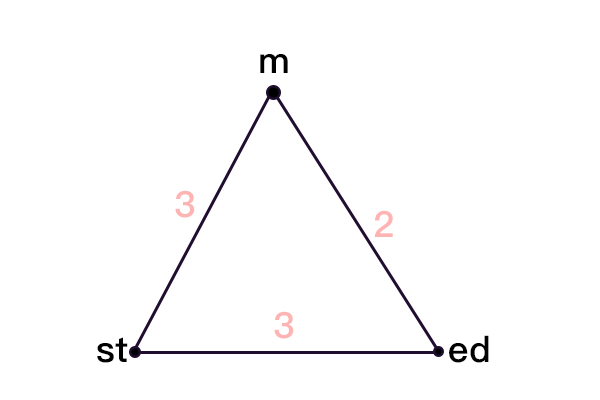
\includegraphics[width=0.6\textwidth]{./pictures/stage3_simplelified.png}
    \caption{简化后的地图}
    \label{fig:simplified3}
\end{figure}
 
整体的可行方案有两种,路线一是由起点直接前往终点,中途不做停留,起,另一种是起点点到矿山尽可能的开采获取资金并在截止时间再到终点,最优情况仅可能在这两种情况取得。这两者的区别在于,路线二相较路线一需要多花两天时间进行行进,但同时前往矿山提供了获得资金的机会。

对于第三关所给出的特殊设定进行分析,不难给出论断:直接前往终点一定会带来更高的收益.理由如下:

考虑最为理想的天气条件,即挖矿与多余行进的日子都为晴朗天气,此时矿山之中的收益达到最大值,多出的两天行进的耗费降到最低。路线二在矿山挖矿的最长时间为$10-3-2=5$(天),每天挖矿获得 200元资金收入,每天消耗的水和食物所需钱数为$3*3*5+4*3*10=165$(元),5 天内可以收益$(200-165)*5=175$(元),多余的两天行进在晴朗天气下消耗的水和食物所需的总金额为 $(3*2*5+4*2*10)*2=220$(元),对比可知,挖矿带来的最大可能收益低于在路上花费的额外开销的最小可能耗费,因此直接前往终点一定会带来更高的收益。

在这样的论断下,玩家仅需要在对于接下来第 1、2、3 s天的天气进行估计,然后进行初始资源的购买。

建立概率模型:

假设晴天出现的概率为 $p$,则高温天气出现的概率为$(1-p)$,天与天之间的天气状况服从独立同分布的两点分布,即某一天的分布与其之前的天气情况无关,$n=3$时,由于三天的天气情况不会对于消耗产生影响,可以认为总共有四种情况:3晴,2晴1高,1晴2高,3高,对应的概率为

以两种天气出现概率相同为例,此时 $p=0.5$,四种天气出现天数组合所对应的概率为:
\begin{table}

\centering

\begin{tabular}{c |c | c | c }
    
      3晴 & 2晴1高 & 1晴2高 & 3高   \\
    \hline
    \hline
      $\frac{1}{8}$ & $\frac{3}{8}$ & $\frac{3}{8}$ & $\frac{1}{8}$ \\
     \hline 
     \hline
     18水+24食 & 30水+34食 &  42水+44食 &  54水+54食 \\

\end{tabular}

\caption{不同天气对应概率与所需最小存活需求物资表}

\end{table}

概率分布如图 \ref{fig:cdf}。

\begin{figure}[htpb]
    \centering
    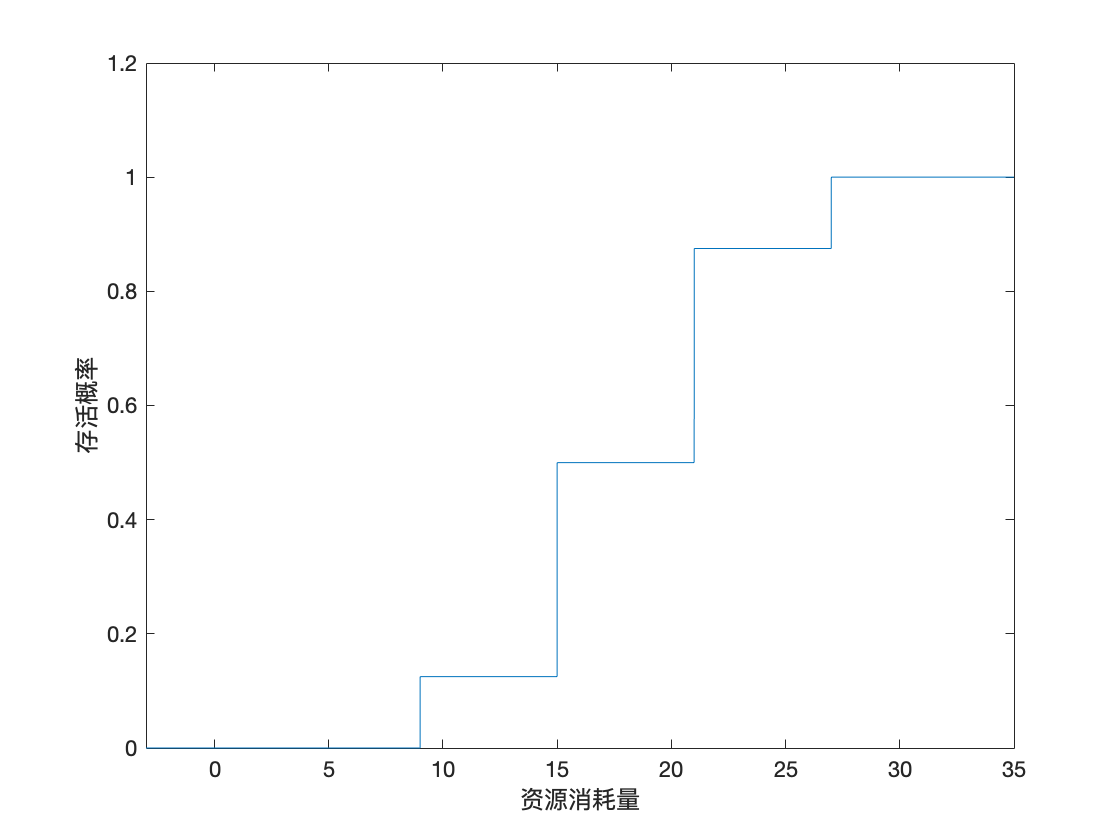
\includegraphics[width=0.8\textwidth]{./pictures/probability.png}
    \caption{资源消耗量的累积分布函数}
    \label{fig:cdf}
\end{figure}

为了保证利益最大化,任何条件下出法都应该仅携带其估计天气状况下的最少资源,,携带任何介于两种方案之间的资源方案既无法带来任何生存概率的提高,反而会由于过量购买在终点以半价卖出而蒙受损失。即按估计天气到达终点将会耗尽所有携带资源,对于以上四种天气对应的最低,携带18水+24食物的最激进方案仅有12.5\%的存活几率,30水+34食物的风险方案有50\%(0.125+0.375)的存活几率,42水+44食物的次保险方案有87.5\%(0.125+0.375+0.375)的存活几率,54水+54食物的最保险方案具有100\%的存活几率。

对于单个玩家,可以在初始时对于自身的生存几率进行一个设定,假设为k,在概率分布图中即可视为目标分位数,寻求生存几率大于该设定值k的最小资源配置方案,如一个玩家追需要保证对安全,生存几率设置为100\%,寻找概率1对应图上的位置,携带54箱水加54箱食物的最保险方案即为其最优选择;对于一个追求刺激的玩家,生存几率设置为70\%,寻找生存概率大于分位数0.7所对应的最低资源配置,即次保险方案是其最合理的选择方案。

\begin{table}

\centering

\begin{tabular}{c || c || c || c }
    
      3晴 & 2晴1高 & 1晴2高 & 3高   \\
    \hline
    \hline
      $\frac{C^{3}_{3}*p^{3}}{2^{3}}$ & $\frac{C^{2}_{3}*p^{2}*(1-p)}{2^{3}}$ & $\frac{C^{1}_{3}*p*(1-p)^{2}}{2^{3}}$ & $\frac{C^{0}_{3}*(1-p)^{3}}{2^{3}}$ \\

\end{tabular}

\caption{天气对应概率}

\end{table}

\subsection{第四关的分析与求解}

\begin{figure}[htpb]
    \centering
    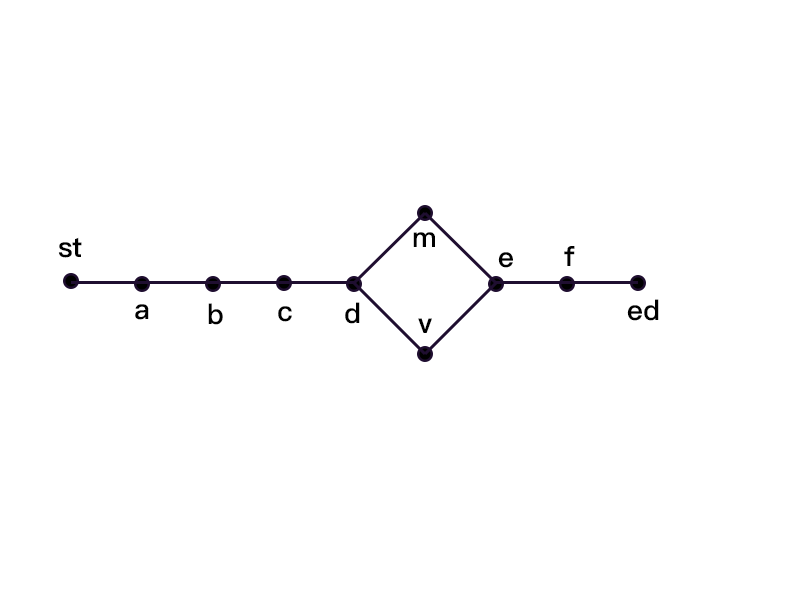
\includegraphics[width=0.8\textwidth]{./pictures/stage4.png}
    \caption{第四关简化后的地图}
    \label{fig:stage4}
\end{figure}

可取启发指标计算公式如下进行计算:

\begin{align*}
    \omega &= \dfrac{2}{t - t_{ed} + 2}\ (l_1 > 0)\\
    \alpha &= \dfrac{2}{a_f - E_f} \cdot \dfrac{2}{a_w - E_w}\\
    \beta &= 10 d_m + 1
.\end{align*}

\subsubsection{在本题中启发函数的设计}

针对本题的地图特例,还应该有下面的性质,可用于检验得到的启发函数是否合理:

\begin{enumerate}
    \item 从起点出发后,启发函数应当引导玩家走向 d,并且一旦到达 d 就不会再有走向 st、a、b、c 的决策出现。因为距离上,d 点相较于上述结点,距离矿山、村庄、终点三个特殊功能结点都更近。不论是生存上还是经济上,d 点都是占优的。
    \item 类似地,一旦玩家到达 e,就绝对不会再有走向 d 的决策出现。
\end{enumerate}

\section{问题三的模型建立与求解}

\subsection{模型准备}
问题三总共有两个小问,问(1)需要对于已知天气条件下给多人进行初步的规划,对于题设条件中多人发生交互的情况进行分析,当有k个玩家同时出现在矿山,挖矿的收益会被k等分,多人出现在同一地点时,购买与同行导致的消耗都会显著上升,对于得到最优解这一最终目标,题设并没有具体说明多人之间是合作关系还是竞争关系,由于竞争关系必然无法避免互相猜疑、恶性竞争等一系列行为,反而对于个体而言期望的收益也会大幅度降低,同时我们保证第0天多人同时在一个地点出发,假设多方有具体的交流机会,通过合作的得到的收益最低的人的最终资金也会大于竞争模型下的个体期望最大值,最优解必然是在消息互通的情况下通过合作获得,即变为多人合作博弈模型。


\subsection{模型建立与求解}
$N=\{1,2,...,n\}$表示局中有n个从起点出发的玩家,总共有$2^{n}$种结盟方式,其集合为N,其对应的功效函数为V(S),即在这种条件下某种结盟T的期望收益,该多人模型是一个具有超可加性的稳定模型,即满足$S,T\in N,S\cap T=\emptyset$ 且$V(S\cup T)\geq V(s)+V(T)$.在互相交流的前提下一定会结成n个人的结盟。

本文尝试给出一种对于n较小情况下的合作模型可取策略,
对于n=2的一般合作模型,给出以下准则:

\begin{enumerate}
    \item 在绝大多数时候,任何多个玩家出现在某位置聚集的情况都会造成巨大的利益损失,可以通过停留或是走分岔路(不是绕路,距离目标特殊地点不发生变化)来避免这样事情的发生。
    \item 在类似5,6这类设定下,高温天停留一天相较于行进所节约的水与食物,大于晴朗天气下所消耗的水与食物总金额的,在时间条件允许的前提下,可以通过高温天原地等待,在晴朗天气进行行进的方式来减小损耗。
    \item 首先运用前四关的方法给出地图在n=1时对应的个人路径最优解,如果个人最优解过程中不经过矿山与村庄,则n=2时最优解为A通过在某位置等候一天达到对于B的跟随状态,然后按最优解进行行动。
    \item 如果地图中只有一个矿山存在,要想得到更高的利润,应该由A按照最优路径行进值矿山进行开采获取资金,B按照前往终点最快路径前往终点往往能带来更大的收益.
    \item 当地图中的矿山数$Mc\geq 2$时,可以类似于关卡3、4,给出以其中不同的矿场为主体开采地点的最优路线图,然后在这样的基础上,两两配对,在基于上述准则1、2的情况下,进行一定的微调,选出能够得到最大收益的一组选项,作为最终的结果.
\end{enumerate}

当$n>2$时,可以通过数学归纳法的方式来解决:

\begin{enumerate}
    \item 如果此时矿山数$Mc\geq n$时,可以按照上述n=2模型之中第5条准则,做出一次$C_{Mc}^{n}$的搜索,并对得到的结果进行微调,选出最大收益的可能.
    \item 如果此时矿山数$Mc\leq n$时,可以令$n-Mc$名玩家类似上述准则4直接前往终点位置,剩余$Mc$名玩家按照更低维度的n=Mc时进行处理(当遇到存在离起点较近的矿山且矿山的基础收益额较高时,可以就具体问题进行微调,使得同一座矿山被多名玩家在不同时间开采).
\end{enumerate}

对于第五关,此时模型中的假设数据与第三关完全相同,前往矿山依旧只能带来负收益,因此,两名玩家的最优选择都是以最快速度前往终点的同时,尽可能避免同时出现在同一个位置,设两名玩家的代号为A,B,晴天和高温对应的符号表示为Q,G;给出以下枚举可能:

\begin{enumerate}
    \item 路径: A:1-5-6-13; B:1-stay-5-6-13;
          总消耗:63水+72食物
    \item 路径: A:1-5-6-13 B:1-4-stay-6-13
         总消耗:57水+67食物
    \item  路径:A:1-5-6-13 B:1-4-7-12-13
        总消耗:66水+76食物
    \item 路径:A:1-5-stay-6-13 B:1-4-stay-stay-6-13
         总消耗:57水+70食物
\end{enumerate}

其他的任意方式都是在如上四种方式的变种,只能通过绕路或多加等待的方式给出新的路径,这些路径的消耗一定超出以上四种本源策略,而在四种策略之中,策略2有效地将二人在第一天分开去向不同地点,保证了不产生4倍的行路消耗的同时,避开了一天高温天,有效地减小了损耗。由此给出第五题在合作前提下的最佳方案:
\begin{enumerate}
    \item A购买30箱水、34箱食物出发,路线为1-5-6-13.
    \item B购买27箱水、33箱食物出发,路线为1-4-stay-6-13.
    \item 到达终点时A收益为-490,到达B时的最终收益-465,群体的最终收益为-955.
\end{enumerate}

第六关由于时间原因并不能够完成其建模,但第四关所对应的模型与程序同时可以进一步地进行一些迁移与拓展,对问题二中的启发函数加入一个新的参数$S_{人}$(沿用该启发函数的符号表示),这个参数为某位置至所有其他人员的最短路径之和,这个数字与$\alpha$成反比,距离越大,潜在的生存概率就越高,与$\beta$成反比,距离越大,潜在的赚钱几率就会越高。该算法需要计算每两个点之间的最短距离,可以用Dijkstra算法先行计算,存储以备确认最短路径之和使用。

\section{模型的评价及推广}

\subsection{模型的优点}

本文提出的启发式策略模型可以里用启发函数设计和选取来精确地描述当前的情景,以文中给出的决策启发函数为例。提供了大量可以进行微调的常数参数部分,每一个常数都可以微调决策函数在某一方面的灵敏度。

\subsection{模型的缺点}

在进行决策的过程之中,物资购买量估计、物资对生存保障情况的估计这样的重要参数是通过给定的天气概率模型来决定的。因此初始的概率模型对于决策过程是否能够保障任务的完成影响极大。不好的概率模型可使决策函数完全失效。

\subsection{改进方法}

第一,如果可以获取更多进行决策之前的天气信息,则可以考虑充分利用信息保证模型的准确度。

第二,寻找其他的估计生存保障程度的方法,如果可以摆脱对概率模型的依赖,则不存在此问题了。

\section{总结与展望}

随着科技的发展,市面上的实时策略游戏愈加丰富多彩,不仅充满了趣味性,更多的起到了益智的作用,使我们思维更为灵活。研究实时策略游戏的攻略不仅有良好的学术价值,可以推动机器学习、神经网络等机器算法的发展,而且有广泛的应用场景,具备良好的商业价值。

麻雀虽小,五脏俱全。本文所涉及的游戏虽小,但却很符合当代人对于该类问题解决方案的寻求,这种稍显简单的游戏分析处理模型可以嵌套于其它较为复杂的系统,进行相关系统的决策。例如,这种实时策略游戏的处理不仅可以用于机器人的行为决策,还能应用于人们日常旅游的出行规划,优化出行方案,使人们的旅行更舒适、更方便。

本文对于穿越沙漠小游戏的决策处理,完美体现了分类讨论的美妙之处,除了天气状况的不同,玩家在不同天气状况下能采取的行为活动也不同,与此同时,食物与水的消耗量以及需求量和购买量都是处于一种动态变化的过程,各种参数耦合在一起,使题目难度加大,更有挑战性和趣味性的同时,也让该游戏超脱于虚拟游戏,与生活实际更为贴合,进而更好地指导我们的日常生活和生产实践。

三道题目各不相同,有一致之处,也有情景的不同,本文根据不同的地图,可以采用不同的规划方式进行处理,或简单,或复杂,但万变不离其宗,总是能找到一个数学模型与其对应,体现了数学的简化之美,令人沉醉。

综上所述,该类实时策略小游戏具有数学之美,在学术性浓厚的同时,也具备良好的趣味性和可迁移性,对于机器人的方案决策以及生活实际都有指导作用,有着良好的商业价值。在后续的学习和工作中,有待于将更多的新理论和新技术融合于此,使其更具备普适性和应用性。

\section{参考文献}

本文所有内容均为原创。

\section{附录}

\subsection{附件清单}
\begin{minted}{text}
.
|-- Result.xlxs
|-- enums.go
|-- go.mod
|-- interactive.go
|-- main.go
|-- modling.exe
|-- stage.gos
|-- stage4.go
|-- stage_parser.go
|-- state_recorder.go
|-- traveler.go
--- stage
    |-- stage1.txt
    |-- stage2.txt
    --- stage4.txt
\end{minted}

\subsection{源代码}

以下程序完全使用 golang 编写,需要打开 go mod 功能后进入 main.go 文件所在的目录进行编译,会得到一个命令行交互程序。该程序根据队员的使用习惯高度定制化,限于篇幅不进行详细描述。

每一个代码块书写一个独立文件的内容,文件名为每个代码块第一行的注释。

% enums.go
\begin{minted}{go}
// enums.go
package main

// NodeType enum type define for representing node type: normal,
// village, mine
type NodeType int8

const (
    normalNode NodeType = iota
    villageNode
    mineNode
    startingNode
    endingNode
)

var specialNodeMap = map[string]NodeType{
    "v": villageNode, "m": mineNode, "s": startingNode, "e": endingNode,
}

func (n NodeType) String() string {
    return []string{"Normal", "Village", "Mine", "Start", "End"}[n]
}

// WeatherType enum for different weather
type WeatherType int8

const (
    highTemp WeatherType = iota
    sunny
    sandStorm
)

var weatherMap = map[string]WeatherType{
    "sun": sunny, "sand": sandStorm, "high": highTemp,
}

func (w WeatherType) String() string {
    return []string{"High Tempreture", "Sunny", "SandStorm"}[w]
}

// ResourceType enum for resource type
type ResourceType int8

const (
    resourceWater ResourceType = iota
    resourceFood
)

var resourceMap = map[string]ResourceType{
    "water": resourceWater, "food": resourceFood,
}
\end{minted}

\hrule

% interactive.go
\begin{minted}{go}
// interactive.go
package main

import (
    "bufio"
    "fmt"
    "os"
    "strconv"
    "strings"
)

var commandMap = map[string]func([]string, *Traveler, *StateRecorder) error{}

func init() {
    commandMap["repeat"] = commandRepeat
    commandMap["undo"] = commandUndo
    commandMap["redo"] = commandRedo
    commandMap["undoto"] = commandUndoUntil
    commandMap["redoto"] = commandRedoUntil
    commandMap["history"] = commandHistory
    commandMap["go"] = commandGoto
    commandMap["log"] = commandLogState
    commandMap["graph-info"] = commandGraphInfo
    commandMap["stage-info"] = commandStageInfo
    commandMap["weather"] = commandWeather
    commandMap["mine"] = commandMining
    commandMap["buy"] = commandBuy
    commandMap["stay"] = commandStay
    commandMap["random-run"] = randomRun
}

func shell(t *Traveler, states *StateRecorder) {
    command := ""
    scanner := bufio.NewScanner(os.Stdin)
    scanner.Split(bufio.ScanLines)
    for command != "quite" {
        fmt.Print(colorYellow, "Traveling> ", colorNone)
        scanner.Scan()
        input := scanner.Text()
        commands := strings.Split(input, ";")
        for _, command := range commands {
            command = strings.TrimSpace(command)
            if len(command) == 0 {
                continue
            }
            parts := strings.Split(command, " ")
            err := singleCommand(command, parts, t, states)
            if err != nil {
                fmt.Println(err)
                continue
            }
        }
    }
}

func singleCommand(command string, parts []string, t *Traveler, states *StateRecorder) error {
    handler, ok := commandMap[parts[0]]
    if !ok {
        return fmt.Errorf("Unknown command `%s`", parts[0])
    }
    fmt.Println()
    err := handler(parts[1:], t, states)
    if err != nil {
        return err
    }
    if parts[0] != "repeat" {
        states.appendCommand(command)
    }
    fmt.Println()
    return nil
}

func commandRepeat(args []string, t *Traveler, states *StateRecorder) error {
    if len(args) < 2 {
        return fmt.Errorf("Not enough argument")
    }
    times, err := strconv.Atoi(args[0])
    if err != nil {
        return err
    }
    for i := 0; i < times; i++ {
        err = singleCommand(strings.Join(args[1:], ""), args[1:], t, states)
        if err != nil {
            return err
        }
    }
    return nil
}

func commandGoto(args []string, t *Traveler, states *StateRecorder) error {
    if !t.ok {
        return fmt.Errorf("Traveler not in normal state")
    }
    if len(args) == 0 {
        return fmt.Errorf("Not enough argument for command")
    }
    for _, arg := range args {
        ok := t.moveTo(arg)
        if !ok {
            return fmt.Errorf("No such node with id '%s'", arg)
        }
    }
    t.checkState()
    states.appendRecord(t)
    commandLogState(args, t, states)
    return nil
}

func commandUndo(args []string, t *Traveler, states *StateRecorder) error {
    if len(args) != 0 {
        return fmt.Errorf("Too much argument")
    }
    err := states.undo(t)
    if err != nil {
        return err
    }
    commandLogState(args, t, states)
    return nil
}

func commandRedo(args []string, t *Traveler, states *StateRecorder) error {
    if len(args) != 0 {
        return fmt.Errorf("Too much argument for command 'back'")
    }
    err := states.redo(t)
    if err != nil {
        return err
    }
    commandLogState(args, t, states)
    return nil
}

func commandUndoUntil(args []string, t *Traveler, states *StateRecorder) error {
    if len(args) != 1 {
        return fmt.Errorf("Wrong number of argument")
    }
    date, err := strconv.Atoi(args[0])
    if err != nil {
        return err
    }
    err = states.undoToDate(t, date)
    if err != nil {
        return err
    }
    commandLogState(args, t, states)
    return nil
}

func commandRedoUntil(args []string, t *Traveler, states *StateRecorder) error {
    if len(args) != 1 {
        return fmt.Errorf("Wrong number of argument")
    }
    date, err := strconv.Atoi(args[0])
    if err != nil {
        return err
    }
    err = states.redoToDate(t, date)
    if err != nil {
        return err
    }
    commandLogState(args, t, states)
    return nil
}

func commandLogState(_ []string, t *Traveler, _ *StateRecorder) error {
    if t == nil {
        return fmt.Errorf("Invalide traveler")
    }
    fmt.Println(t.String())
    return nil
}

func commandHistory(args []string, t *Traveler, states *StateRecorder) error {
    for i, command := range states.commands[:states.currPos] {
        fmt.Printf("%d: %s\n", i+1, command)
    }
    return nil
}

func commandMining(args []string, t *Traveler, states *StateRecorder) error {
    if !t.ok {
        return fmt.Errorf("Traveler not in normal state")
    }
    ok := t.mining()
    if !ok {
        return fmt.Errorf("You have to go to mine to do this")
    }
    t.checkState()
    states.appendRecord(t)
    commandLogState(args, t, states)
    return nil
}

func commandBuy(args []string, t *Traveler, states *StateRecorder) error {
    if !t.ok {
        return fmt.Errorf("Traveler not in normal state")
    } else if len(args) > 2 {
        return fmt.Errorf("too much arguments")
    }
    var (
        foodAmount  int
        waterAmount int
    )
    for _, arg := range args {
        parts := strings.Split(arg, ":")
        if len(parts) != 2 {
            return fmt.Errorf("Wrong sperator usage in argument '%s'", arg)
        }
        value, err := strconv.Atoi(parts[1])
        if err != nil {
            return err
        }
        if parts[0] == "food" {
            foodAmount = value
        } else if parts[0] == "water" {
            waterAmount = value
        }
    }
    ok := t.buyResource(foodAmount, waterAmount)
    if !ok {
        return fmt.Errorf("You have to go to village to do this or buy resource for the first time at starting point")
    }
    t.checkState()
    states.appendRecord(t)
    commandLogState(args, t, states)
    return nil
}

func commandGraphInfo(_ []string, t *Traveler, _ *StateRecorder) error {
    if t == nil || t.Graph == nil {
        return fmt.Errorf("Invalid traveler")
    }
    fmt.Println(t.Graph.String())
    return nil
}

func commandStageInfo(_ []string, t *Traveler, _ *StateRecorder) error {
    if t == nil || t.Stage == nil {
        return fmt.Errorf("Invalid traveler")
    }
    fmt.Println(t.Stage.String())
    return nil
}

func commandWeather(_ []string, t *Traveler, _ *StateRecorder) error {
    if t == nil || t.Stage == nil {
        return fmt.Errorf("Invalid traveler")
    }
    for i, weather := range t.Stage.weatherList {
        fmt.Printf("%d: %s\n", i, weather)
    }
    return nil
}

func commandStay(args []string, t *Traveler, states *StateRecorder) error {
    t.stay()
    t.checkState()
    states.appendRecord(t)
    commandLogState(args, t, states)
    return nil
}

\end{minted}

\hrule

% main.go
\begin{minted}{go}
// main.go
package main

import (
    "flag"
    "log"
)

const (
    colorNone   string = "\033[0m"
    colorRed           = "\033[1;31m"
    colorGreen         = "\033[32m"
    colorYellow        = "\033[33m"
)

var stageFile = flag.String("stage", "stage.txt", "stage file to read from")
var initDate = flag.Int("date", 0, "Intial date of process")
var initPosition = flag.String("pos", "st", "Initial position of traveler")
var initMoney = flag.Int("money", -1, "Initial budget for travler")
var initWater = flag.Int("water", 0, "Initial water for travler")
var initFood = flag.Int("food", 0, "Initial food for travler")
var notFirstBuy = flag.Bool("first", false, "Initial state of first state")
var isInverse = flag.Bool("inverse", false, "Inverse traveling process, cumulate resource from current place")

func main() {
    flag.Parse()
    t := newTraveler(*stageFile)
    if t == nil {
        log.Println("Traveler initialize failed")
        return
    }
    travelerInit(t)
    states := newRecorder(t)
    shell(t, states)
}

func travelerInit(t *Traveler) {
    t.date = *initDate
    t.position = *initPosition
    if *initMoney >= 0 {
        t.money = *initMoney
    }
    t.food = *initFood
    t.water = *initWater
    t.loadSpace = t.loadSpace - t.food*t.resourceWeight[resourceFood] + t.water*t.resourceWeight[resourceWater]
    t.firstBuy = !*notFirstBuy
}
\end{minted}

\hrule

% stage_parser.go
\begin{minted}{go}
// stage_parser.go
package main

import (
    "errors"
    "fmt"
    "log"
    "strconv"
    "strings"
)

// ParserMap is a map recording parser for each section
var ParserMap = map[string]func(*Stage, string) error{}

func init() {
    ParserMap["day count"] = parseDayCount
    ParserMap["load"] = parseLoad
    ParserMap["base budget"] = parseBudget
    ParserMap["base income"] = parseBaseIncome
    ParserMap["weight & base price"] = parseWeightAndBasePrice
    ParserMap["base cost"] = parseBaseCost
    ParserMap["node count"] = parseNodeCount
    ParserMap["special node"] = parseSpecial
    ParserMap["adjacent releation"] = parseAdj
    ParserMap["weather"] = parseWeather
    ParserMap["path weight"] = parsePathWeight
}

func parseDayCount(s *Stage, line string) error {
    count, err := strconv.Atoi(line)
    if err != nil {
        return err
    }
    s.dayCount = count
    return nil
}

func parseLoad(s *Stage, line string) error {
    count, err := strconv.Atoi(line)
    if err != nil {
        return err
    }
    s.load = count
    return nil
}

func parseBudget(s *Stage, line string) error {
    count, err := strconv.Atoi(line)
    if err != nil {
        return err
    }
    s.baseBudget = count
    return nil
}

func parseBaseIncome(s *Stage, line string) error {
    count, err := strconv.Atoi(line)
    if err != nil {
        return err
    }
    s.baseIncome = count
    return nil
}

func parseNodeCount(s *Stage, line string) error {
    count, err := strconv.Atoi(line)
    if err != nil {
        return err
    }
    s.nodeCount = count
    return nil
}

func parseWeightAndBasePrice(s *Stage, line string) error {
    parts := strings.Split(line, ":")
    if len(parts) != 3 {
        return errors.New("Wrong Sperator Usage")
    }
    kind, ok := resourceMap[parts[0]]
    if !ok {
        return errors.New("Unknown weather type")
    }
    weight, err := strconv.Atoi(parts[1])
    if err != nil {
        return err
    }
    s.resourceWeight[kind] = weight
    price, err := strconv.Atoi(parts[2])
    if err != nil {
        return err
    }
    s.resourceBasePrice[kind] = price
    return nil
}

func parseBaseCost(s *Stage, line string) error {
    parts := strings.Split(line, ":")
    if len(parts) != 3 {
        return errors.New("Wrong Sperator Usage")
    }
    weatherKind, ok := weatherMap[parts[0]]
    if !ok {
        return fmt.Errorf("Unknown weather type %s", parts[0])
    }
    resourceKind, ok := resourceMap[parts[1]]
    if !ok {
        return fmt.Errorf("Unknown resource type %s", parts[1])
    }
    cost, err := strconv.Atoi(parts[2])
    if err != nil {
        return err
    }
    s.resourceBaseCost[weatherKind][resourceKind] = cost
    return nil
}

func parseSpecial(s *Stage, line string) error {
    parts := strings.Split(line, ":")
    if len(parts) != 2 {
        return errors.New("Wrong Sperator Usage")
    }
    id, kind := parts[0], parts[1]
    specialKind, ok := specialNodeMap[kind]
    if !ok {
        return errors.New("Error node type")
    }
    s.special[id] = specialKind
    return nil
}

func parseAdj(s *Stage, line string) error {
    parts := strings.Split(line, ":")
    if len(parts) != 2 {
        return errors.New("Wrong Sperator Usage")
    }
    id, neighbourStr := parts[0], parts[1]
    adjList, ok := s.adjacents[id]
    if !ok {
        adjList = []string{}
    }
    for _, neighbour := range strings.Split(neighbourStr, ",") {
        adjList = append(adjList, neighbour)
    }
    s.adjacents[id] = adjList
    return nil
}

func parseWeather(s *Stage, line string) error {
    weathers := strings.Split(line, ",")
    for _, weather := range weathers {
        weatherKind, ok := weatherMap[weather]
        if !ok {
            log.Println("Unknown weather type:", weather)
            return errors.New("Unknown weather type")
        }
        s.weatherList = append(s.weatherList, weatherKind)
    }
    return nil
}

func parsePathWeight(s *Stage, line string) error {
    parts := strings.Split(line, ":")
    if len(parts) != 2 {
        return errors.New("Wrong sperator usage")
    }
    weight, err := strconv.Atoi(parts[1])
    if err != nil {
        return err
    }
    nodeIDs := strings.Split(parts[0], ",")
    if len(parts) != 2 {
        return errors.New("Wrong sperator usage")
    }
    for i := 0; i < 2; i++ {
        j := 1 - i
        weightMap, ok := s.weightMap[nodeIDs[i]]
        if !ok {
            weightMap = map[string]int{}
        }
        weightMap[nodeIDs[j]] = weight
        s.weightMap[nodeIDs[i]] = weightMap
    }
    return nil
}
\end{minted}

\hrule

% stage.go
\begin{minted}{go}
// stage.go
package main

import (
    "bufio"
    "bytes"
    "fmt"
    "log"
    "math/rand"
    "os"
    "strings"
)

// Node is a single node in graph
type Node struct {
    id         string
    neighbour  map[*Node]struct{}
    nodeType   NodeType
    pathWeight map[string]int
}

func newNode(id string) *Node {
    return &Node{id, map[*Node]struct{}{}, normalNode, map[string]int{}}
}

// Graph graph object
type Graph struct {
    starting *Node
    ending   *Node
    nodes    map[string]*Node
}

func newGraph() *Graph {
    return &Graph{nil, nil, map[string]*Node{}}
}

func (g *Graph) appendAdj(id1 string, id2 string) error {
    node1, ok := g.nodes[id1]
    if !ok {
        node1 = newNode(id1)
        g.nodes[id1] = node1
    }
    node2, ok := g.nodes[id2]
    if !ok {
        node2 = newNode(id2)
        g.nodes[id2] = node2
    }
    node1.neighbour[node2] = struct{}{}
    node2.neighbour[node1] = struct{}{}
    return nil
}

func (g *Graph) String() string {
    buf := bytes.NewBufferString("")
    for _, node := range g.nodes {
        fmt.Fprintf(buf, "Node ID: %s\nNode Type: %s\n", node.id, node.nodeType)
        fmt.Fprintf(buf, "Neighbour: ")
        for neighbour := range node.neighbour {
            fmt.Fprintf(buf, "%s ", neighbour.id)
        }
        fmt.Fprintf(buf, "\n--------------------\n")
    }
    return buf.String()
}

// Stage store graph info in txt file, includeing: node count, stating & ending point,
// special node, adjacent releasion etc.
type Stage struct {
    dayCount          int
    load              int
    baseBudget        int
    baseIncome        int
    resourceWeight    [2]int
    resourceBasePrice [2]int
    resourceBaseCost  [3][2]int
    nodeCount         int
    special           map[string]NodeType
    adjacents         map[string][]string
    weightMap         map[string]map[string]int
    weatherList       []WeatherType
}

func (s *Stage) String() string {
    buf := bytes.NewBufferString("")
    fmt.Fprintln(buf, "Day Count:", s.dayCount)
    fmt.Fprintln(buf, "Load:", s.load)
    fmt.Fprintln(buf, "Budget:", s.baseBudget)
    fmt.Fprintln(buf, "Income:", s.baseBudget)
    fmt.Fprintln(buf, "Weight:", s.resourceWeight)
    fmt.Fprintln(buf, "Price:", s.resourceBasePrice)
    return buf.String()
}

func stageFromFile(filePath string) (*Stage, error) {
    file, err := os.Open(filePath)
    if err != nil {
        return nil, err
    }
    scanner := bufio.NewScanner(file)
    scanner.Split(bufio.ScanLines)
    var (
        line    string
        section string
        parser  func(*Stage, string) error
        hasIt   bool
    )
    stage := new(Stage)
    stage.special = map[string]NodeType{}
    stage.adjacents = map[string][]string{}
    stage.weightMap = map[string]map[string]int{}
    stage.weatherList = []WeatherType{}
    for scanner.Scan() {
        line = strings.TrimSpace(scanner.Text())
        if len(line) == 0 {
            continue
        } else if strings.HasPrefix(line, "- ") {
            section = line[2:]
            parser, hasIt = ParserMap[section]
            if !hasIt {
                log.Println("Unknown section name:", section)
            }
            continue
        } else if !hasIt {
            continue
        }
        err := parser(stage, line)
        if err != nil {
            log.Printf(
                "Section '%s' parsing error while parsing: %s\n", section, line,
            )
            return nil, err
        }
    }
    fmt.Println("Stage read from file:", filePath)
    return stage, nil
}

func (s *Stage) makeGraph() *Graph {
    g := newGraph()
    for id, neighbours := range s.adjacents {
        g.nodes[id] = newNode(id)
        for _, n := range neighbours {
            g.appendAdj(id, n)
        }
    }
    for id, kind := range s.special {
        g.nodes[id].nodeType = kind
        if kind == startingNode {
            g.starting = g.nodes[id]
        } else if kind == endingNode {
            g.ending = g.nodes[id]
        }
    }
    for id, neightbours := range s.weightMap {
        node := g.nodes[id]
        for idn, weight := range neightbours {
            node.pathWeight[idn] = weight
        }
    }
    return g
}

func (s *Stage) randWeather(pSun float64, pHigh float64, pSand float64) {
    pHigh += pSun
    pSand += pHigh
    pSun /= pSand
    pHigh /= pSand
    pSand = 1
    var (
        value   float64
        weather WeatherType
    )
    for i := 0; i < s.dayCount; i++ {
        value = rand.Float64()
        switch {
        case value < pSun:
            weather = sunny
        case value < pHigh:
            weather = highTemp
        default:
            weather = sandStorm
        }
        s.weatherList = append(s.weatherList, weather)
    }
}
\end{minted}

\hrule

% stage4.go
\begin{minted}{go}
// stage.go
package main

import (
    "fmt"
    "math/rand"
)

var foodExpect = map[string]map[string]float64{}
var waterExpect = map[string]map[string]float64{}

func randWeather(pSun float64, pHigh float64, pSand float64, dayCount int) []WeatherType {
    pSand += pHigh
    pSun /= pSand
    pHigh /= pSand
    pSand = 1
    weatherList := []WeatherType{}
    var (
        value   float64
        weather WeatherType
    )
    for i := 0; i < dayCount; i++ {
        value = rand.Float64()
        switch {
        case value < pSun:
            weather = sunny
        case value < pHigh:
            weather = highTemp
        default:
            weather = sandStorm
        }
        weatherList = append(weatherList, weather)
    }
    return weatherList
}

func randomRun(_ []string, t *Traveler, state *StateRecorder) error {
    pSun, pHigh, pSand := 0.5, 0.4, 0.1
    loopCount := 30
    for i := 0; i < loopCount; i++ {
        t.Stage.weatherList = randWeather(pSun, pHigh, pSand, 8)
        for id := range t.Graph.nodes {
            for _, pos := range []string{"v", "m", "ed"} {
                resetState(t, id)
                t.moveTo(pos)
                addToExpectation(&foodExpect, id, pos, float64(t.food))
                addToExpectation(&waterExpect, id, pos, float64(t.water))

            }
        }
    }
    fmt.Println("Food Expectation")
    for id, special := range foodExpect {
        fmt.Println(id)
        for pos, value := range special {
            value /= float64(loopCount)
            fmt.Printf("\t%s: %.2f\n", pos, value)
            foodExpect[id][pos] = value
        }
    }
    fmt.Println("Water Expectation")
    for id, special := range waterExpect {
        fmt.Println(id)
        for pos, value := range special {
            value /= float64(loopCount)
            fmt.Printf("\t%s: %.2f\n", pos, value)
            waterExpect[id][pos] = value
        }
    }
    return nil
}

func resetState(t *Traveler, pos string) {
    t.date = 0
    t.position = pos
    t.food = 0
    t.water = 0
    t.loadSpace = t.Stage.load
    t.money = t.Stage.baseBudget
}

func addToExpectation(expectation *map[string]map[string]float64, id string, pos string, value float64) {
    expMap, ok := (*expectation)[id]
    if !ok {
        expMap = map[string]float64{}
    }
    expMap[pos] -= value
    (*expectation)[id] = expMap
}
\end{minted}

\hrule

% state_recorder.go
\begin{minted}{go}
// state_recorder.go
package main

import (
    "fmt"
    "strings"
)

// StateRecorder is a history state for traveling process
type StateRecorder struct {
    currPos  int // current position in record stack
    commands []string
    states   []Traveler
}

func newRecorder(t *Traveler) *StateRecorder {
    return &StateRecorder{0, []string{}, []Traveler{*t}}
}

func (r *StateRecorder) appendRecord(t *Traveler) {
    r.currPos++
    if r.currPos < len(r.states) {
        r.states[r.currPos] = *t
    } else {
        r.states = append(r.states, *t)
    }
}

func (r *StateRecorder) appendCommand(command string) {
    skipPrefix := []string{"redo", "undo", "history", "log"}
    for _, prefix := range skipPrefix {
        if strings.HasPrefix(command, prefix) {
            return
        }
    }
    if r.currPos > 0 && r.currPos-1 < len(r.commands) {
        r.commands[r.currPos-1] = command
    } else {
        r.commands = append(r.commands, command)
    }
}

func (r *StateRecorder) undo(t *Traveler) error {
    if r.currPos == 0 {
        return fmt.Errorf("No older states")
    }
    r.currPos--
    r.readState(t)
    return nil
}

func (r *StateRecorder) redo(t *Traveler) error {
    if r.currPos == len(r.states)-1 {
        return fmt.Errorf("No newer states")
    }
    r.currPos++
    r.readState(t)
    return nil
}

func (r *StateRecorder) undoToDate(t *Traveler, date int) error {
    if r.currPos == 0 {
        return fmt.Errorf("No older states")
    }
    pos := r.currPos
    for pos > -1 && r.states[pos].date != date {
        pos--
    }
    if pos >= 0 {
        r.currPos = pos
    } else {
        return fmt.Errorf("Invalid date")
    }
    r.readState(t)
    return nil
}

func (r *StateRecorder) redoToDate(t *Traveler, date int) error {
    if r.currPos == len(r.states)-1 {
        return fmt.Errorf("No newer state")
    }
    pos := r.currPos
    for pos > -1 && r.states[pos].date != date {
        pos++
    }
    if pos >= 0 {
        r.currPos = pos
    } else {
        return fmt.Errorf("Invalid date")
    }
    r.readState(t)
    return nil
}

func (r *StateRecorder) readState(t *Traveler) {
    old := r.states[r.currPos]
    t.date = old.date
    t.position = old.position
    t.loadSpace = old.loadSpace
    t.money = old.money
    t.water = old.water
    t.food = old.food
    t.ok = old.ok
    t.firstBuy = old.firstBuy
}
\end{minted}

\hrule

% traveler.go
\begin{minted}{go}
// traveler.go
package main

import (
    "bytes"
    "fmt"
    "log"
)

// Traveler is object that record traveling state, like position, date, resource
type Traveler struct {
    *Stage
    *Graph
    date          int
    position      string
    loadSpace     int // load space left for resource
    money         int
    water         int
    food          int
    ok            bool // wheather traveler is in a normal state
    firstBuy      bool
    heuristicFunc func(*Traveler) string
}

func newTraveler(stageFile string) *Traveler {
    stage, err := stageFromFile(stageFile)
    if err != nil {
        log.Println(err)
        return nil
    }
    graph := stage.makeGraph()
    return &Traveler{
        Stage:     stage,
        Graph:     graph,
        date:      0,
        position:  graph.starting.id,
        loadSpace: stage.load,
        money:     stage.baseBudget,
        water:     0,
        food:      0,
        ok:        true,
        firstBuy:  true,
    }
}

func (t *Traveler) String() string {
    buf := bytes.NewBufferString("")
    var state string
    if t.ok {
        state = colorGreen + "Ok" + colorNone
    } else {
        state = colorRed + "Error" + colorNone
    }
    fmt.Fprintf(buf, "State: %s\n", state)
    if t.date < 30 {
        fmt.Fprintf(buf, "Weather Tommorrow: %s\n", t.Stage.weatherList[t.date])
    }
    fmt.Fprint(buf, "| Date | Position | Load Space |  Money  | Food | Water |\n")
    fmt.Fprintf(buf, "|%6d|%10s|%12d|%9d|%6d|%7d|", t.date, t.position, t.loadSpace, t.money, t.food, t.water)
    return buf.String()
}

func (t *Traveler) checkState() bool {
    inTime := (t.date < t.dayCount) || (t.date == t.dayCount && t.position == t.ending.id)
    t.ok = inTime && t.loadSpace >= 0 // && t.water >= 0 && t.food >= 0
    return t.ok
}

func (t *Traveler) stay() bool {
    t.consumeResource(1)
    t.date++
    return true
}

func (t *Traveler) moveTo(id string) bool {
    _, ok := t.nodes[id]
    if !ok {
        return false
    }
    distance, ok := t.nodes[t.position].pathWeight[id]
    if !ok {
        distance = 1
    }
    for distance > 0 {
        if t.weatherList[t.date] == sandStorm {
            t.consumeResource(1)
        } else {
            t.consumeResource(2)
            distance--
        }
        t.date++
        // fmt.Println(t.date, distance)
    }
    t.position = id
    return true
}

func (t *Traveler) buyResource(foodAmount int, waterAmount int) bool {
    // if t.starting.id == t.position && t.firstBuy || t.nodes[t.position].nodeType == villageNode {
    // 	t.firstBuy = false
    // } else {
    // 	// return false
    // }
    cost := foodAmount*t.resourceBasePrice[resourceFood] + waterAmount*t.resourceBasePrice[resourceWater]
    if !t.firstBuy {
        cost *= 2
    }
    weight := foodAmount*t.resourceWeight[resourceFood] + waterAmount*t.resourceWeight[resourceWater]
    t.money -= cost
    t.loadSpace -= weight
    t.food += foodAmount
    t.water += waterAmount
    t.firstBuy = false
    return true
}

func (t *Traveler) mining() bool {
    if t.nodes[t.position].nodeType != mineNode {
        return false
    }
    t.consumeResource(3)
    t.money += t.baseIncome
    t.date++
    return true
}

func (t *Traveler) consumeResource(multiplier int) {
    var weather WeatherType
    if *isInverse {
        weather = t.weatherList[t.date-1]
    } else {
        weather = t.weatherList[t.date]
    }
    foodCost := t.resourceBaseCost[weather][resourceFood] * multiplier
    waterCost := t.resourceBaseCost[weather][resourceWater] * multiplier
    t.food -= foodCost
    t.water -= waterCost
    if t.loadSpace < t.Stage.load {
        t.loadSpace += foodCost*t.resourceWeight[resourceFood] + waterCost*t.resourceWeight[resourceWater]
    }
}

func (t *Traveler) moveWithHeuristic() {
    if t.heuristicFunc == nil {
        return
    }
    t.moveTo(t.heuristicFunc(t))
}
\end{minted}

\end{document}
